\subsection{Cloud-Based Key Management Systems}\label{sec:key_management:cloud}

%Other relevant aspects requiring a careful evaluation are the cryptographic architecture --- intended as the set of hardware and software entities providing cryptographic services within a system --- and the choice of which cryptographic ciphers to employ, their configuration, and key types; 
%often, all of these aspects are handled by an automated \textbf{\gls{kms}} --- that is, a dedicated system for the management of cryptographic keys and their metadata \cite{barker_recommendation_2019_p2} --- whose usefulness has been widely recognized \cite{barker_framework_2013,barker_profile_2015}. 



Considering the sensitivity and importance of cryptographic material --- and private and secret keys in particular --- \glspl{kms} have been traditionally developed and used within (the trusted boundaries of) organizations. However, with the advent of Cloud computing and the digitalization of technological infrastructures, the outsourcing of services to the Cloud involved \glspl{kms} as well, mainly due to better scale and performance and reduced costs and complexity \cite{csa_key_2020}, but also the fact that \glspl{kms} offered by well-established Cloud providers usually provide higher security than most on-premises \glspl{kms} \cite{csa_recommendations_2021}. Furthermore, the outsourcing of technical services such as \glspl{kms} allows for more straightforward management and seamless integration with business and Cloud services in general, enabling a wide array of security features such as automatic encryption for data at rest and in transit. Moreover, Cloud-based \glspl{kms} often provide geographic distribution and redundancy, guaranteeing high availability and (almost effortless) disaster recovery.

\remarkBlock{Definition of cloud computing}{Cloud computing is defined by \gls{nist} as ``a model for enabling ubiquitous, convenient, on-demand network access to a shared pool of configurable computing resources (e.g., networks, servers, storage, applications, and services) that can be rapidly provisioned and released with minimal management effort or service provider interaction'' \cite{mell_nist_2011}.}

Fostered by a high demand on the part of organizations, in the last years major Cloud providers have been developing feature-rich \glspl{kms}, suitable for use by a heterogeneous set of organizations ranging from financial services, pharmaceuticals, and government bodies \cite{csa_key_2020}. Besides, the integration of \glspl{kms} with \gls{iam} services (see S8-CSC-D1 in \Cref{sec:intro:scope}) offers a complete and unified solution to (most of) the technological needs of organizations --- such as authentication, authorization, and data protection. Below, we first discuss the 4 main architectures for Cloud-based \glspl{kms}, and then provide a more concrete description of \glspl{kms} --- and other relevant services --- offered by the 3 major Cloud providers (i.e., \gls{aws}, Google, Microsoft).



\subsubsection{Architectures for Cloud-Based Key Management Systems}\label{sec:cloud:architectures}

\begin{figure}[t!]
	\begin{center}
		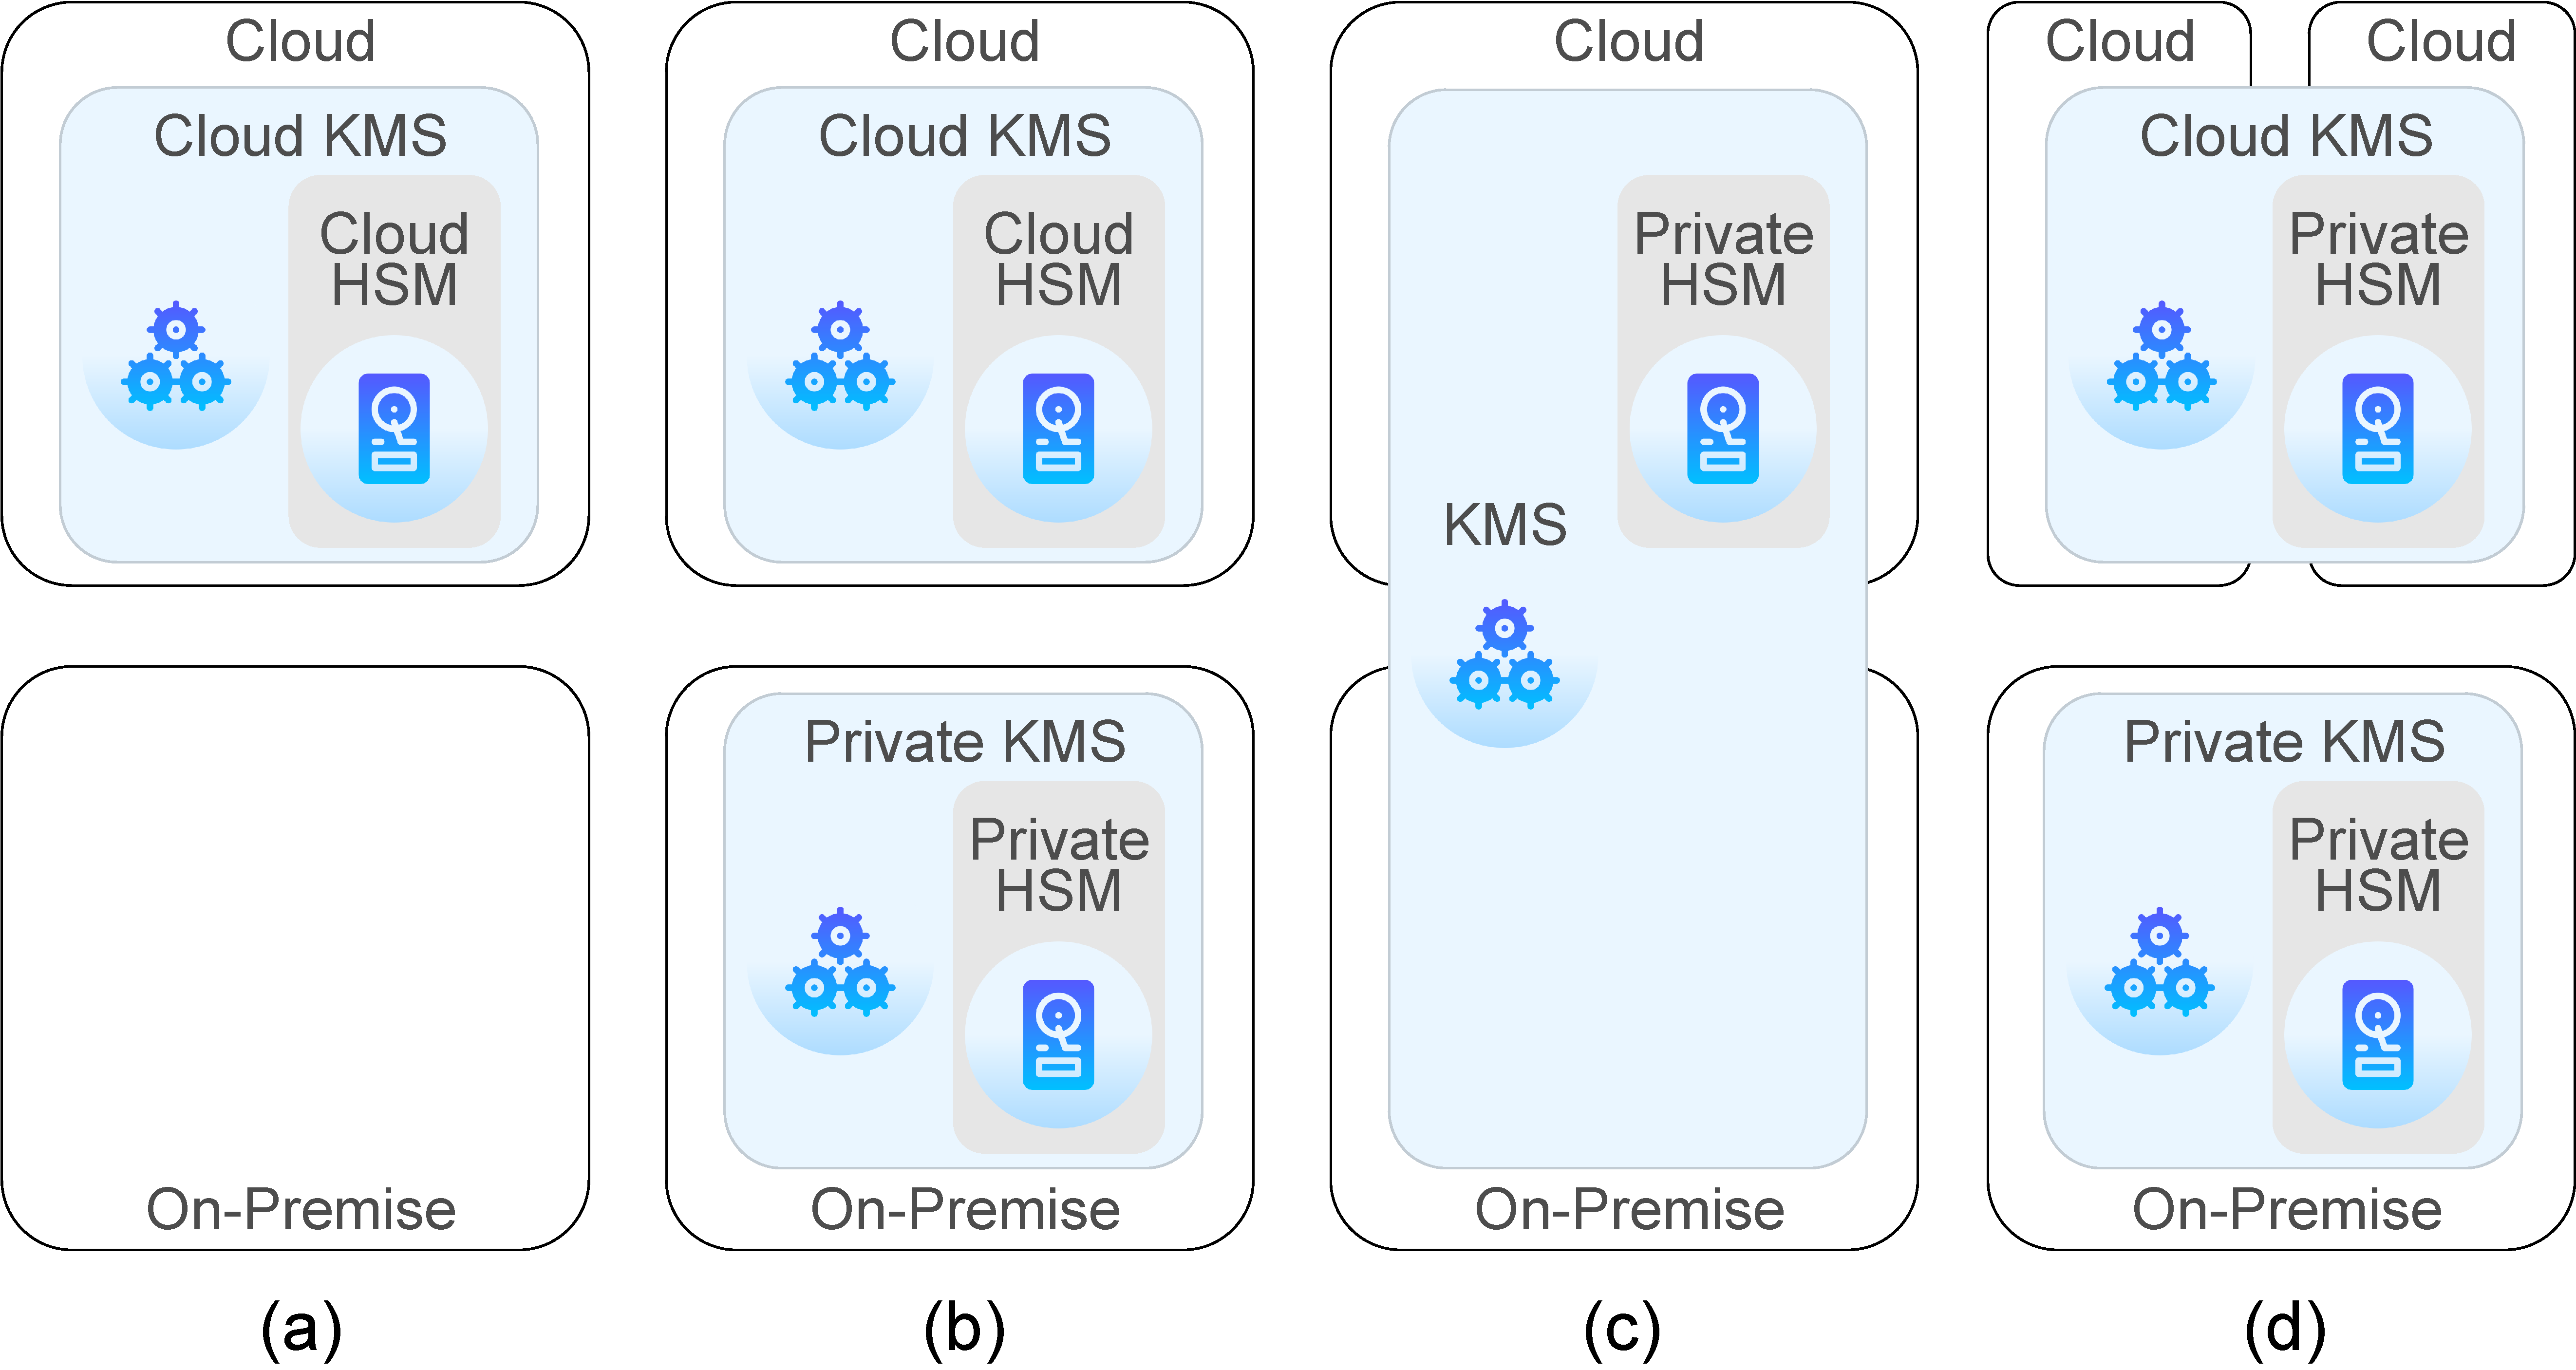
\includegraphics[width=1\linewidth]{resources/pdf/kms.pdf}
		\caption{\gls{kms} Architectures in the Cloud}
		\label{fig:kms}
	\end{center}
\end{figure}

As discussed in \cite{csa_key_2020} and shown in \Cref{fig:kms}, there are 4 main architectures with which an organization can interact with Cloud-based \glspl{kms}, which we discuss below (note that the use of \glspl{hsm} is strongly recommended in the context of \glspl{kms}). Intuitively, each architecture has its advantages and drawbacks, which organizations should carefully assess to identify the most suitable architecture for (the security, business, and regulatory requirements of) their scenarios. We report the properties of each architecture in \Cref{table:cloud_based_kms_architectures}, where a full, half, and empty circle (i.e., $\fullcirc$, $\halfcirc$, $\emptycirc$) mean that the corresponding property is fully achieved, partially achieved or not achieved by the corresponding architecture, respectively.

\begin{table}[!b]
	\centering
	\small
	\setlength{\tabcolsep}{1.75pt}
	\def\arraystretch{1.075}
	\rowcolors{0}{cloud}{white}
	\caption{Properties of Cloud-Based Key Management Systems Architectures}
	\newcolumntype{Y}{>{\centering\arraybackslash}X}
	\begin{tabularx}{\textwidth}{l|YYYY}
		
		\toprule
		
		\multicolumn{1}{c|}{\multirow{2}{*}\textbf{Property}} &
		\multicolumn{4}{c}\textbf{Cloud-based \gls{kms}} \\
		
		~ &
		\multicolumn{1}{c}\textbf{Pure} &
		\multicolumn{1}{c}\textbf{Combined} &
		\multicolumn{1}{c}\textbf{Hybrid} &
		\multicolumn{1}{c}\textbf{Multiple} \\
		
		\hline
		
		Transparency of the \gls{kms} 				& \emptycirc 	& \halfcirc 	& \fullcirc 	& \halfcirc 	\\
		Control over the \gls{kms} 					& \emptycirc 	& \halfcirc 	& \fullcirc 	& \halfcirc 	\\
		Portability (No Lock-In) 					& \emptycirc 	& \emptycirc 	& \fullcirc 	& \fullcirc 	\\
		Availability								& \halfcirc 	& \halfcirc 	& \halfcirc 	& \fullcirc 	\\
		Scalability									& \fullcirc 	& \fullcirc 	& \emptycirc 	& \fullcirc 	\\
		Performance									& \fullcirc 	& \fullcirc 	& \emptycirc 	& \fullcirc 	\\
		Interoperability with Other Cloud Providers & \emptycirc 	& \emptycirc 	& \emptycirc 	& \fullcirc 	\\
		Low Latency									& \fullcirc 	& \fullcirc 	& \emptycirc 	& \halfcirc 	\\
		Low Cost									& \fullcirc 	& \halfcirc 	& \emptycirc 	& \emptycirc 	\\
		Low Complexity (Fast Adoption)				& \fullcirc 	& \halfcirc 	& \emptycirc 	& \emptycirc 	\\
		Ease in Management							& \fullcirc 	& \halfcirc 	& \emptycirc 	& \emptycirc 	\\
		Prone to Satisfy Regulatory Requirements	& \emptycirc 	& \halfcirc 	& \fullcirc 	& \halfcirc 	\\
		Ease of SLA Definition and Enforcement		& \fullcirc 	& \halfcirc 	& \emptycirc 	& \halfcirc 	\\
		Seamless Support from Cloud Providers		& \fullcirc 	& \fullcirc 	& \halfcirc 	& \halfcirc 	\\
		Data Protection from Cloud Providers		& \emptycirc 	& \emptycirc 	& \fullcirc 	& \halfcirc 	\\
		Low Knowledge on \gls{kms} Required  		& \fullcirc 	& \halfcirc 	& \emptycirc 	& \emptycirc 	\\
		
		\bottomrule
		
	\end{tabularx}
	\label{table:cloud_based_kms_architectures}
\end{table}


% description
% advantages (``On the one hand'')
% disadvantages (``On the other hand'')
% when the architecture is recommended (``This architecture is usually recommended when'')
\paragraph*{Pure Cloud-Based Key Management System.}

\Cref{fig:kms}(a) shows an architecture where the \gls{kms} and the corresponding \gls{hsm} are managed entirely by a single Cloud provider --- ideally, the same provider offering the business services for which the \gls{kms} is used. The pure Cloud-based \gls{kms} is also known as ``Cloud-native \gls{kms}''. On the one hand, this architecture has intrinsically low latency, high performance, and high scalability, and it is the simplest to adopt, as it requires little knowledge on key management on the part of the organizations --- indeed, the Cloud provider manages all (or at least the majority of) aspects of the key management lifecycle. On the other hand, by delegating the \gls{kms} to the Cloud provider, organizations have little or no control over cryptographic keys (e.g., key lengths, cryptoperiod), cryptographic ciphers, or their configuration --- which may sometimes even be opaque to the organizations, complicating the achievement of compliance requirements. Moreover, (the design and functioning of) \gls{kms} offered by Cloud providers usually differ from each other, possibly leading to strong lock-in. This architecture is usually recommended when the organizations lack (or do not desire to acquire) specific expertise on \glspl{kms} and wish to achieve rapid deployment of business services \cite{csa_key_2020}. For a more detailed and concrete discussion on how to choose, plan, and deploy a pure Cloud-based \gls{kms} --- as well as technical, operational, regulatory, legal, and final recommendations --- we refer the interested reader to \cite{csa_recommendations_2021}.


\paragraph*{Combined Cloud-Based Key Management System.}

The architecture shown in \Cref{fig:kms}(b) extends the architecture in \Cref{fig:kms}(a) by allowing the exchange of cryptographic material between an on-premise \gls{kms} and a Cloud-based \gls{kms}; typically, cryptographic material (e.g., master keys) is created and exported from the former and then imported onto the latter --- it seldom happens the other way around \cite{csa_key_2020}. The two \glspl{kms} are thus distinct, that is, no integration is expected. The combined Cloud-based \gls{kms} is also known as ``Cloud-native \gls{kms} with an external key origin''. On the one hand, organizations have now some control over how cryptographic material is generated (e.g., what software and hardware are used). Moreover, this architecture has intrinsically low latency, high performance, high scalability, and little impact on \glspl{sla} with the Cloud provider. On the other hand, organizations are still limited by the design and functioning of Cloud-based \glspl{kms}, which requires organizations to configure the on-premise \gls{kms} (and private \gls{hsm}) to preserve compatibility --- while still entailing strong lock-in. Furthermore, organizations need some knowledge of \glspl{kms}. Finally, organizations should be aware of eventual modifications (e.g., addition of critical metadata) that Cloud providers apply on cryptographic material when imported on the Cloud-based \gls{kms} \cite{csa_key_2020} --- hence, transparency is still limited.\footnote{Service encryption with Microsoft Purview Customer Key (\url{https://docs.microsoft.com/en-us/microsoft-365/compliance/customer-key-overview?view=o365-worldwide})} This architecture is usually recommended when organizations want to control (at least the) the generation of cryptographic material or need to fulfill specific regulatory requirements that cannot be achieved by using Cloud-based \gls{kms} only --- such as \gls{byok} (see \Cref{sec:cloud:models}). For a more detailed and concrete discussion on how to choose, plan, and deploy a combined Cloud-based \gls{kms} --- as well as technical, operational, regulatory, legal, and final recommendations --- we refer the interested reader to \cite{csa_recommendations_2021_2}.


\paragraph*{Hybrid Cloud-Based Key Management System.}

The architecture in \Cref{fig:kms}(c) shows a \gls{kms} logically spanning from the organization on-premise to the Cloud provider; in other words, functions of the \gls{kms} are used from both on-premise and the Cloud. This architecture follows either the ``Bring-Your-Own-\gls{hsm}'' or the ``\gls{hsm}-as-a-Service'' models:\footnote{The \gls{cla} --- a not-for-profit organization with the mission to educate and promote the use of best practices for security in the Cloud --- is currently working (November 2023) on a white paper tentatively entitled ``\gls{hsm}-as-a-Service: Use Cases, Considerations, and Best Practices''; for more information, see \url{https://cloudsecurityalliance.org/artifacts/hsm-as-a-service-use-cases-considerations-and-best-practices/}} the former means that an organization provides a physical \gls{hsm} that is hosted in the Cloud, while the latter means that the Cloud provider provisions an \gls{hsm} solely for use by the organization \cite{csa_key_2020}. The hybrid Cloud-based \gls{kms} is also known as ``Cloud-native \gls{kms} using external \glspl{kms}''. On the one hand, organizations have full control over the \gls{kms}, the key management lifecycle, and its configuration (recall the concepts explained in \Cref{sec:key_management}) while preventing strong lock-in. On the other hand, this architecture has high cost and limited performance, scalability, and latency. Moreover, this architecture requires the (often complex) definition of \glspl{sla} with the Cloud provider on the use of the \gls{kms} and the \gls{hsm} --- especially in case of incidents. Furthermore, organizations need deep knowledge of \glspl{kms}. This architecture is usually recommended when organizations want full control over the \gls{kms}, need to fulfill specific regulatory requirements that cannot be achieved by adopting other architectures --- such as \gls{cyok} (see \Cref{sec:cloud:models}) --- or must protect their data even from Cloud providers themselves (see \Cref{sec:cloud:models}). As a final remark, note that this architecture is not always supported by Cloud providers (e.g., in 2020, only \gls{aws} and Microsoft provided support for this architecture \cite{csa_key_2020}). For a more detailed and concrete discussion on how to choose, plan, and deploy a hybrid Cloud-based \gls{kms} --- as well as technical, operational, regulatory, legal, and final recommendations --- we refer the interested reader to \cite{csa_recommendations_2022}.


\paragraph*{Multiple Cloud-Based Key Management System.}

The architecture shown in \Cref{fig:kms}(d) illustrated a combined \gls{kms} where the Cloud-based \gls{kms} spans two or more Cloud providers. The multiple Cloud-based \gls{kms} is also known as ``Multi-Cloud \glspl{kms}''. On the one hand, this architecture provides high portability, fault tolerance, and scalability --- mainly due to the use of several Cloud providers. On the other hand, organizations need both deep knowledge of both \glspl{kms} and their functioning as offered by multiple Cloud providers. Also, the complexity of the architecture entails higher costs due to longer design and deployment time. This architecture is usually recommended when the business services of organizations already span multiple Cloud providers, or if organizations need to satisfy specific and complex regulatory requirements. 



\subsubsection{Cloud Providers Offering Key Management Systems Services}\label{sec:cloud:providers}

The first Cloud-based \gls{kms} service was the \gls{aws} Key Management Service, released in late 2014.\footnote{Document history - AWS Key Management Service (\url{https://docs.aws.amazon.com/kms/latest/developerguide/dochistory.html})} Since then, many other Cloud providers implemented and released \glspl{kms}, making proper \glspl{sdk} readily available to organizations. Below, we briefly describe Cloud-based \glspl{kms} and related services offered by 3 major Cloud providers, namely \gls{aws}, Google, and Microsoft.

\remarkBlock{Change velocity of cloud-based \glspl{kms}}{Cloud computing is known for its fast pacing and rapid evolution of products and services; intuitively, this characteristic applies to Cloud-based \glspl{kms} and related services as well. In other words, these often change, and it is therefore recommended to refer to the latest documentation for complete, accurate, and updated information. The content of \Cref{sec:cloud:providers} --- which is to be intended as an overview --- is updated as of December 2023.}


\paragraph*{Amazon Web Services.}

\gls{aws} offers two main services related to Cloud-based \gls{kms}:

\begin{itemize}
	\item \textbf{\gls{aws} Key Management Service}\footnote{Encryption Cryptography Signing - AWS Key Management Service (\url{https://aws.amazon.com/kms/})}: a managed service allowing organizations to handle the key management lifecycle (see \Cref{sec:key_management}) using \glspl{hsm} certified under \gls{fips} 140-2 level 3 (see \Cref{sec:hardware}). The \gls{aws} Key Management Service integrates with most other \gls{aws} services, such as \gls{aws} \gls{s3} --- for encryption of data at rest --- \gls{aws} \gls{iam} --- for authentication and authorization through the definition and enforcement of fine-grained \gls{abac} policies --- and \gls{aws} CloudTrail\footnote{Api Logs - AWS CloudTrail (\url{https://aws.amazon.com/cloudtrail/})} --- for monitoring and auditing key usages. Finally, the \gls{aws} Key Management Service allows organizations to import cryptographic material and synchronize with external \gls{hsm} (i.e., combined Cloud-based \gls{kms}, as discussed in \Cref{sec:cloud:architectures});
	\item \textbf{\gls{aws} CloudHSM}\footnote{Security HSM - AWS CloudHSM (\url{https://aws.amazon.com/cloudhsm/})}: a managed service offering \glspl{hsm}-as-a-Service (recall the corresponding definition in \Cref{sec:cloud:architectures}), employing \glspl{hsm} certified under \gls{fips} 140-2 level 3. CloudHSM allows organizations to manage cryptographic keys --- accessible only by the organizations themselves --- by creating a cluster of \glspl{hsm} spread across multiple \gls{aws} availability zones in a region for high availability and automatic load balancing. CloudHSM does not interoperate directly with on-premises \glspl{hsm}.
\end{itemize}

The Custom Key Store feature\footnote{Custom key stores - AWS Key Management Service (\url{https://docs.aws.amazon.com/kms/latest/developerguide/custom-key-store-overview.html})} combines the controls provided by CloudHSM with the integration and ease of use of the \gls{aws} Key Management Service. In other words, an organization can configure its CloudHSM cluster and then use it from the \gls{aws} Key Management Service as a dedicated key store for keys rather than the default key store. Intuitively, the organization is then responsible for the key management lifecycle of keys generated within the CloudHSM cluster (e.g., key rotation should be performed manually).


\paragraph*{Google.}

Google offers two main services related to Cloud-based \gls{kms} in the Google Cloud suite of Cloud Services:

\begin{itemize}
	\item \textbf{Cloud Key Management Service}:\footnote{Cloud Key Management Service overview | Cloud KMS Documentation (\url{https://cloud.google.com/kms/docs/key-management-service})} a managed service allowing organizations to handle the key management lifecycle (see \Cref{sec:key_management}) using either software-based cryptographic modules certified under \gls{fips} 140-2 level 1 or \glspl{hsm} certified under \gls{fips} 140-2 level 3 with Google Cloud \gls{hsm}.\footnote{Cloud HSM | Cloud KMS Documentation (\url{https://cloud.google.com/kms/docs/hsm})} The Cloud Key Management Service integrates with most other Google Cloud services, such as Cloud \gls{iam}\footnote{Identity and Access Management | IAM | Google Cloud (\url{https://cloud.google.com/iam})} --- for authentication and authorization through the definition and enforcement of fine-grained \gls{abac} policies --- and Cloud Audit Logging\footnote{Cloud Audit Logs overview (\url{https://cloud.google.com/logging/docs/audit})} --- for monitoring and auditing key usages; encryption for data at rest is enabled by default. Finally, the Cloud Key Management Service allows organizations to import cryptographic material and synchronize with external \gls{hsm} (i.e., combined Cloud-based \gls{kms}, as discussed in \Cref{sec:cloud:architectures});
	\item \textbf{Cloud \gls{ekm}}:\footnote{Cloud External Key Manager | Cloud KMS Documentation (\url{https://cloud.google.com/kms/docs/ekm})} a managed service --- released in early access in September 2023 --- allowing to indirectly use cryptographic keys managed by an external \gls{kms} in Google Cloud services (i.e., similar to the combined Cloud-based \gls{kms}, as discussed in \Cref{sec:cloud:architectures}). In other words, keys are never used, cached, or stored within the Google Cloud services, and instead Cloud \gls{ekm} directly invokes the \glspl{api} of the external \gls{kms} --- as it happens in \gls{hyok} models (see \Cref{sec:cloud:models}). This implies that data is always encrypted before being sent to the Cloud, while decryption of data always happens within the external \gls{kms}.
\end{itemize}


\paragraph*{Microsoft Azure.}

Microsoft offers two main services related to Cloud-based \gls{kms} in the Azure Cloud platform:

\begin{itemize}
	\item \textbf{Key Vault}\footnote{Key Vault | Microsoft Azure (\url{https://azure.microsoft.com/en-us/products/key-vault})}: a managed service for the management of generic secrets --- hence, also cryptographic keys. Key Vault has two service tiers: standard, which encrypts with a software key, and premium, which includes the use of \glspl{hsm} certified under \gls{fips} 140-2 level 3;
	\item \textbf{Azure Managed, Dedicated, and Payment \gls{hsm}}\footnote{Overview of Key Management in Azure | Microsoft Learn (\url{https://learn.microsoft.com/en-us/azure/security/fundamentals/key-management})}: a set of 3 managed services offering \glspl{hsm}-as-a-Service (recall the corresponding definition in \Cref{sec:cloud:architectures}), employing \glspl{hsm} certified under FIPS 140-2 level 3. Azure Managed \gls{hsm} is managed by Azure, while the organization is responsible for Azure Dedicated and Payment \gls{hsm}; Azure Dedicated \gls{hsm} is general purpose, while Azure Payment \gls{hsm} is specific for applications in financial services.\footnote{How to choose the right key management solution - How to choose between Azure Key Vault, Azure Managed HSM, Azure Dedicated HSM, and Azure Payment HSM | Microsoft Learn (\url{https://learn.microsoft.com/en-us/azure/security/fundamentals/key-management-choose})}
\end{itemize}

In summary, all 3 Cloud providers offer services related to Cloud-based \gls{kms}. However, \gls{aws} and Google seem to have the most articulated and consolidated services, while Microsoft still lacks a complete \gls{kms}. Note that all 3 Cloud providers claim that no one, including their employees, can retrieve keys from \glspl{hsm}: this may be reasonable by considering that Cloud providers are motivated to avoid legal and reputational damages associated with unauthorized data access and voluntarily allow inspections by third-party auditors.\footnote{Cloud encryption key management: how can Swiss organizations protect their data outside their premises? (\url{https://www2.deloitte.com/ch/en/pages/technology/articles/cloud-encryption-key-management.html})}



\subsubsection{Key Management Models for the Cloud}\label{sec:cloud:models}

As discussed in \Cref{sec:cloud:architectures,sec:cloud:providers}, cryptographic keys can be managed (e.g., generated, used) differently depending on the chosen Cloud-based \glspl{kms} architecture and \gls{kms} Cloud service. In particular, we identify 3 relevant aspects in this regard: ownership, control, and possession --- which correspond to who owns, controls the lifecycle, and physically keeps cryptographic keys (and data, in general). Although ownership of keys is always of the organization (i.e., the customer of the Cloud for which the keys were created), the level of control and possession may vary. For this reason, in the last years, 3 key management models for the Cloud emerged, based on how organizations manage (some aspects of) the key management lifecycle (e.g., generation) externally with respect to Cloud-based \gls{kms} and related services (e.g., using an on-premise \gls{kms} with a dedicated \gls{hsm}):

\begin{itemize}
	\item \textbf{\gls{byok}}: in this model (often also called ``customer-supplied encryption keys''), keys are generated by organizations and imported onto the Cloud for use --- as it happens in the combined Cloud-based \gls{kms} architecture (see \Cref{sec:cloud:architectures}) --- resulting in seamless integration with Cloud services but also the loss of ownership over the keys. Indeed, in \gls{byok}, the Cloud provider has access to private and secret keys;
	\item \textbf{\gls{cyok}}: in this model, keys are generated by organizations and imported onto the Cloud for use --- as it happens in the hybrid Cloud-based \gls{kms} architecture(see \Cref{sec:cloud:architectures}). Although in \gls{byok} cryptographic keys reside within the Cloud, the Cloud provider has no access to private and secret keys (at least theoretically);
	\item \textbf{\gls{hyok}}: in this model, organizations retain full control and ownership over keys, which are never used, cached, or stored in the Cloud (e.g., as it happens in the Cloud \gls{ekm} described in \Cref{sec:cloud:providers}).
\end{itemize}

As is usually the case, there is no key management model that is the most suitable for (the security, business, and regulatory requirements of) all scenarios. Instead, the choice of which model to adopt should be taken on a case-by-case basis. For instance, for most Cloud services following the \gls{saas} pattern (e.g., emails, managed database, analytics services), the Cloud provider must have access to plaintext data; therefore, the \gls{cyok} and \gls{hyok} models are hardly compatible with \gls{saas} services. On the other hand, if an organization requires to preserve the confidentiality of its data even with respect to the Cloud provider, the \gls{byok} model may not be a suitable choice --- especially when combined with dedicated cryptographic constructions such as \gls{cac} \cite{berlato_formal_2022,berlato_end_2022}. Other aspects to consider are further regulatory and compliance requirements, existing key management practices, and the level of control and visibility for keys desired by organizations.

\remarkBlock{Debate around key management models for the cloud}{The acronyms \gls{byok}, \gls{cyok}, and \gls{hyok} originated first as marketing terms and, at the time of writing, there is no official standard or widely agreed upon definition for their semantics; therefore, some deem these terms --- and, in particular, their use --- to be pointless or even confusing, and suggest instead to avoid them entirely \cite{csa_key_2020}.}
